\section{Introduction}
\label{sec:intro}

With the rapid growth of world population and the loss of arable land, there is an increasing desire to improve the yield and quality of crops.  Key to increasing yields is gaining understanding of the genetic mechanisms that influence plant growth~\cite{doos2002population}.
%
A classic genetic approach is to produce a diverse population of mutant lines, grow them either in growth chambers with simulated environmental conditions or directly in the field, visually observe the plants during the growth period, and finally identify plant morphological or physiological patterns that tightly associate with key growth factors~\cite{houle2010phenomics}.
%
While many factors can be assessed quantitatively, which is essential for high-throughput study, one of the bottleneck in this research pipeline is plant visual phenotyping~\cite{walter2015plant}.

\begin{figure*}
\begin{centering}
\begin{tabular}{@{}c c c c c}
%\begin{tabular}{lllllllll}
(a) &
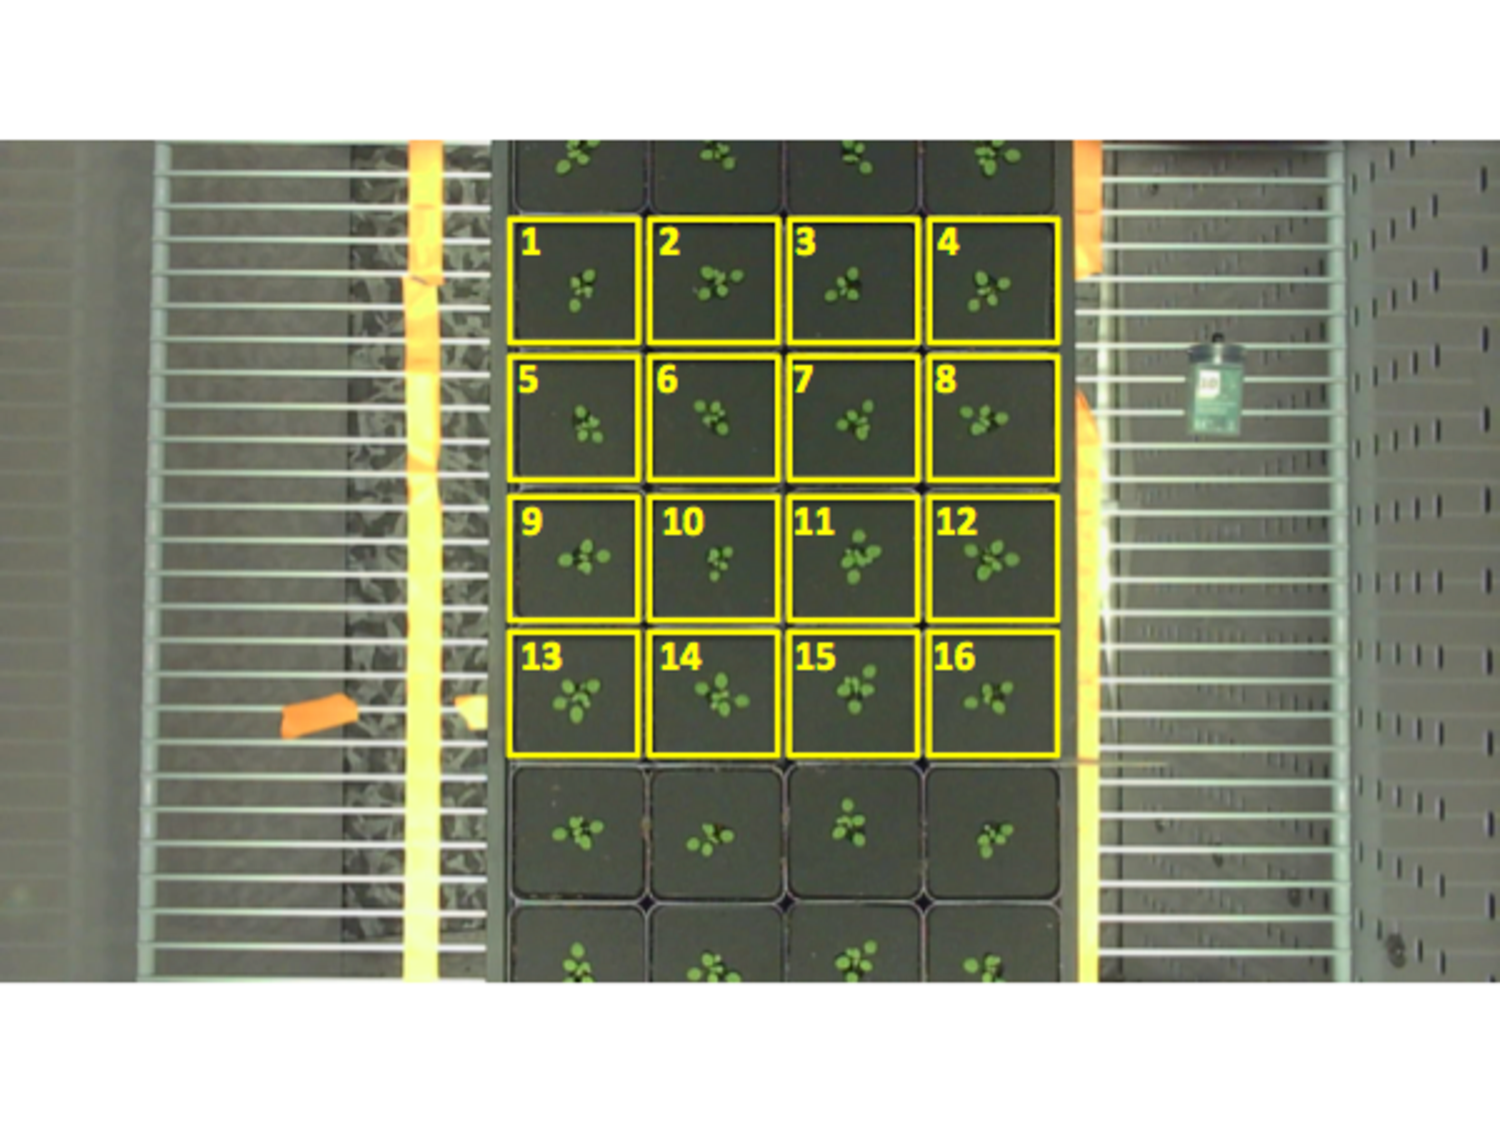
\includegraphics[width=.23\textwidth]{Figures/FourModalities/A_rgb}&
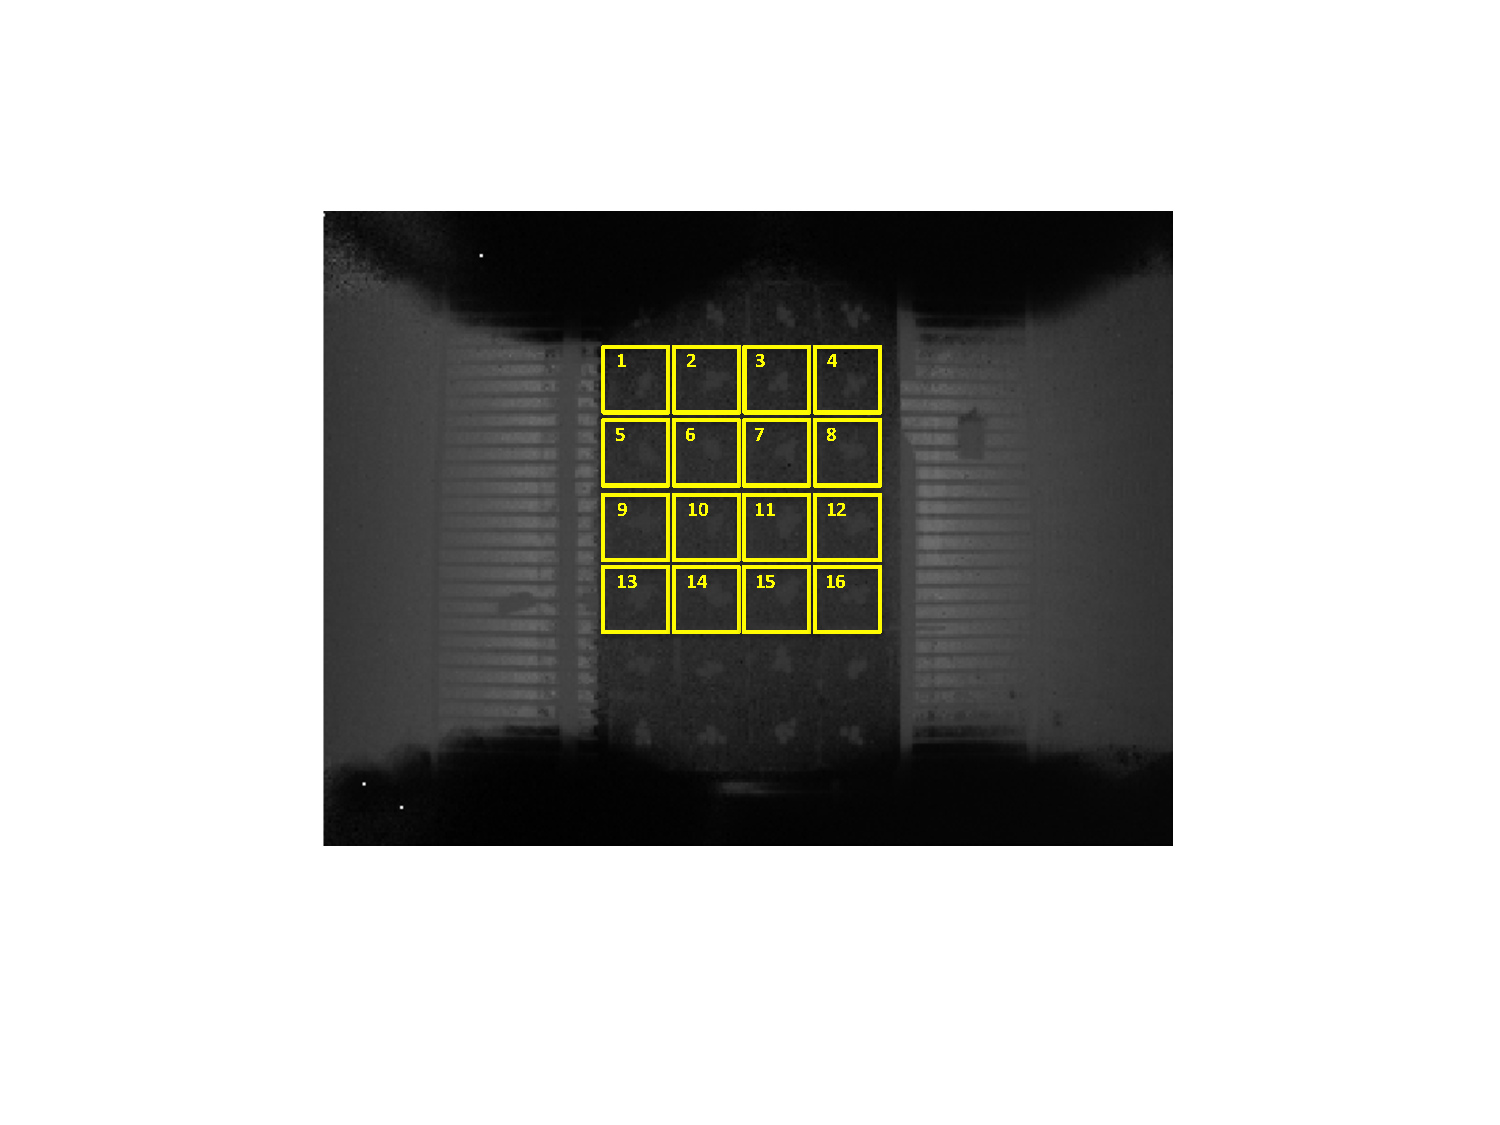
\includegraphics[width=.23\textwidth]{Figures/FourModalities/A_depth}&
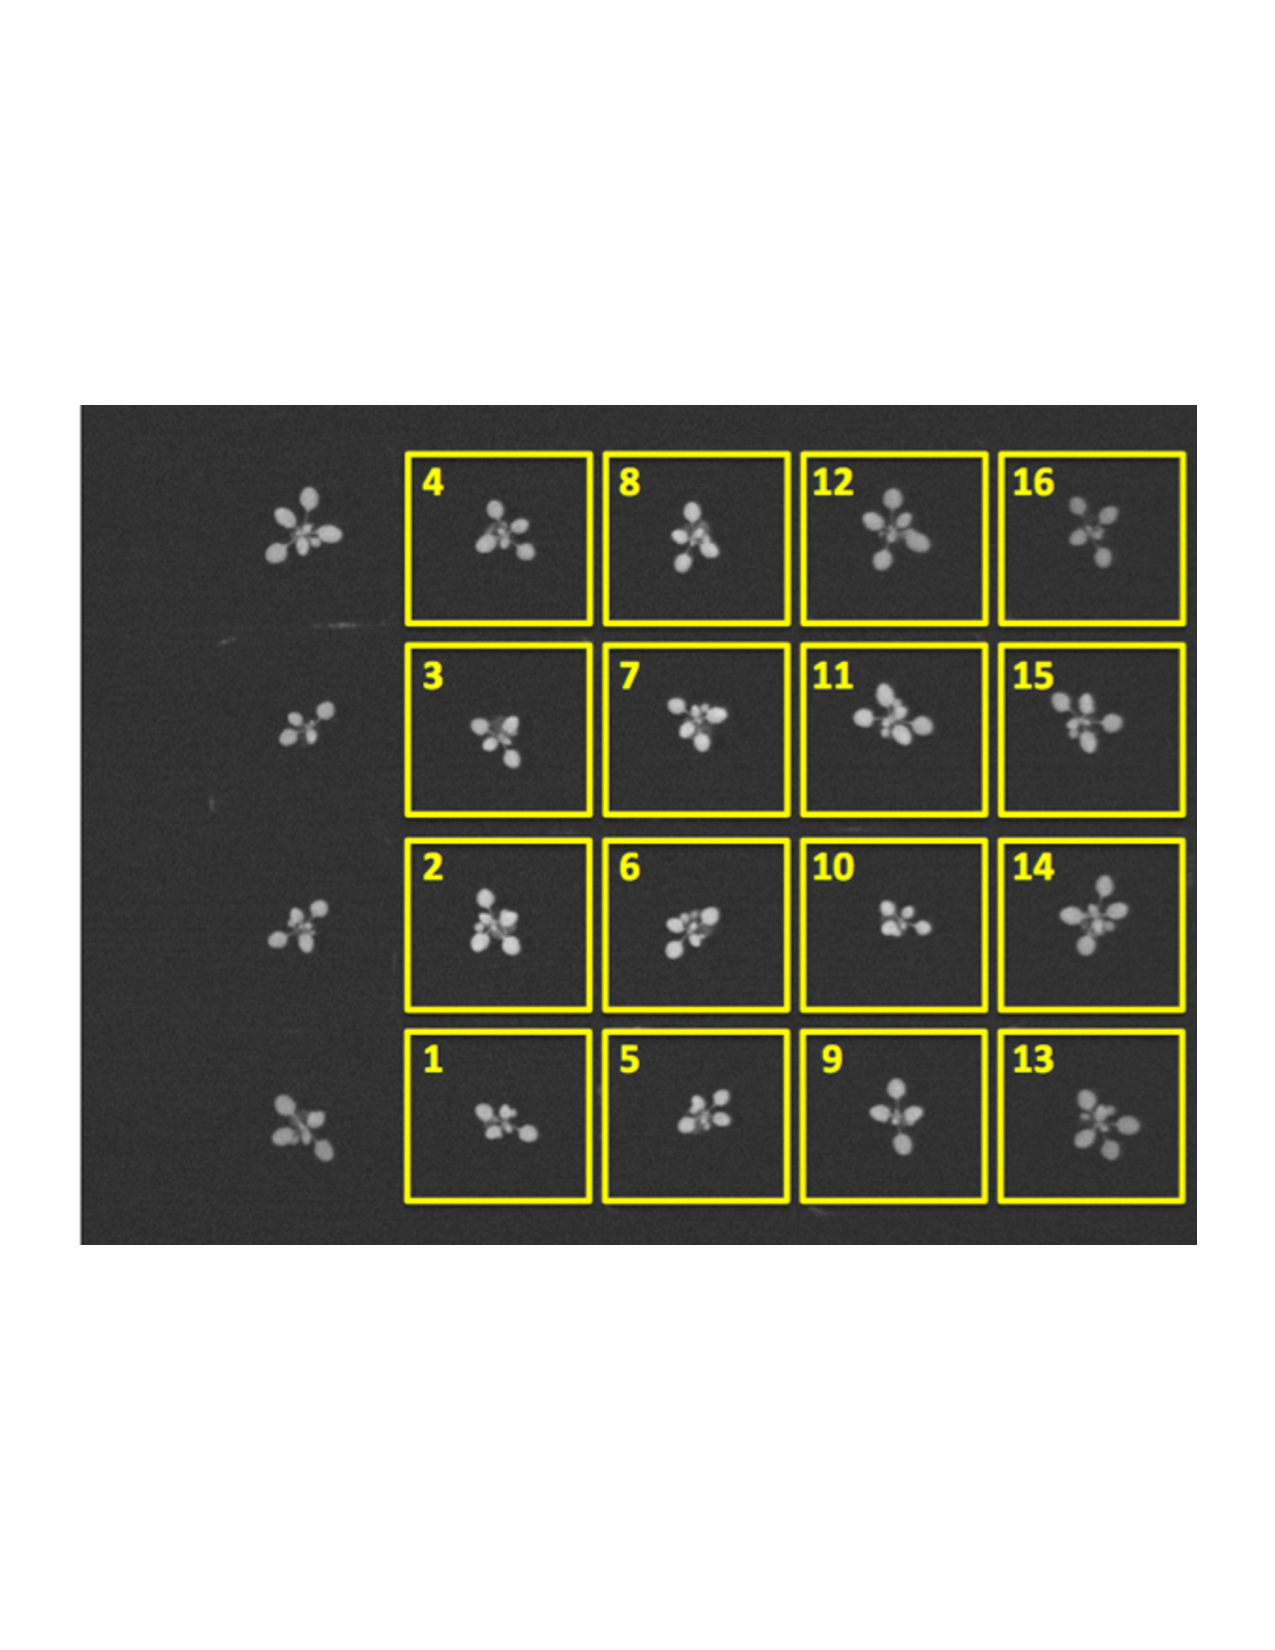
\includegraphics[width=.23\textwidth]{Figures/FourModalities/A_fmp}&
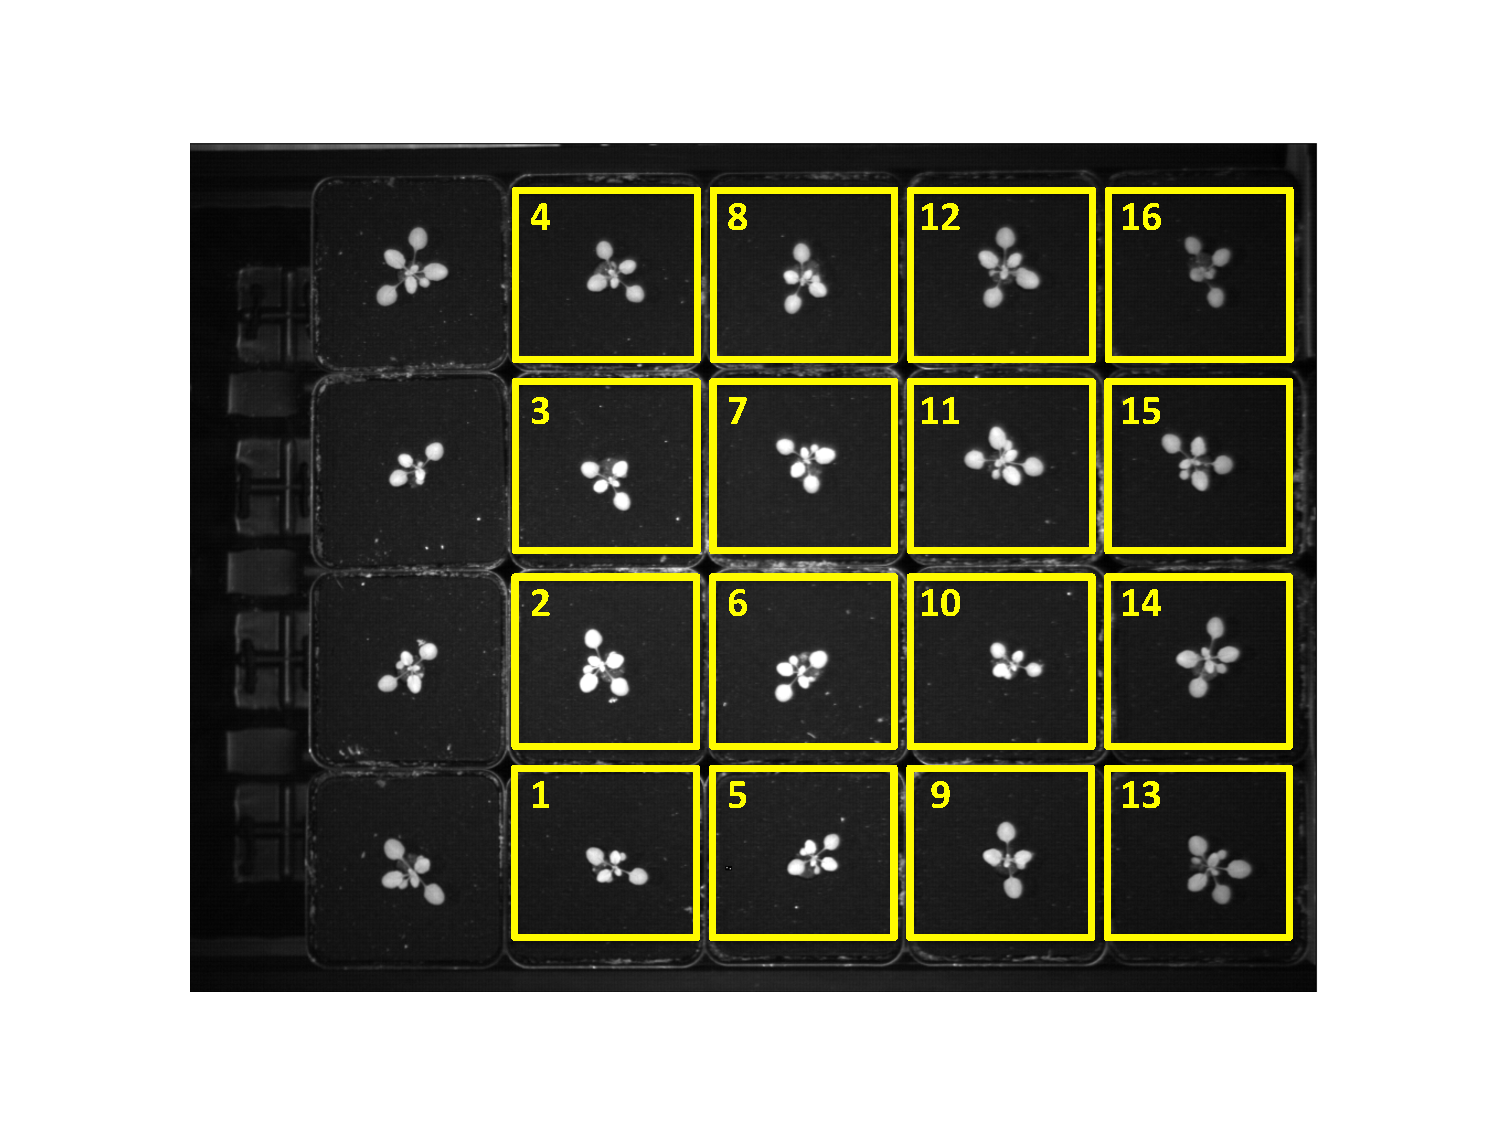
\includegraphics[width=.23\textwidth]{Figures/FourModalities/A_ir}\\
(b) &
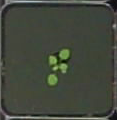
\includegraphics[width=.1\textwidth]{Figures/FourModalities/A1_rgb}&
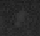
\includegraphics[width=.1\textwidth]{Figures/FourModalities/A1_depth}&
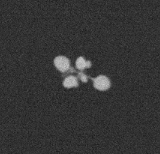
\includegraphics[width=.1\textwidth]{Figures/FourModalities/A1_fmp}&
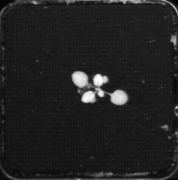
\includegraphics[width=.1\textwidth]{Figures/FourModalities/A1_ir}\\
%Arabidopsis: RGB & Arabidopsis: depth & Arabidopsis: fluorescence & Arabidopsis: IR \\
(c) &
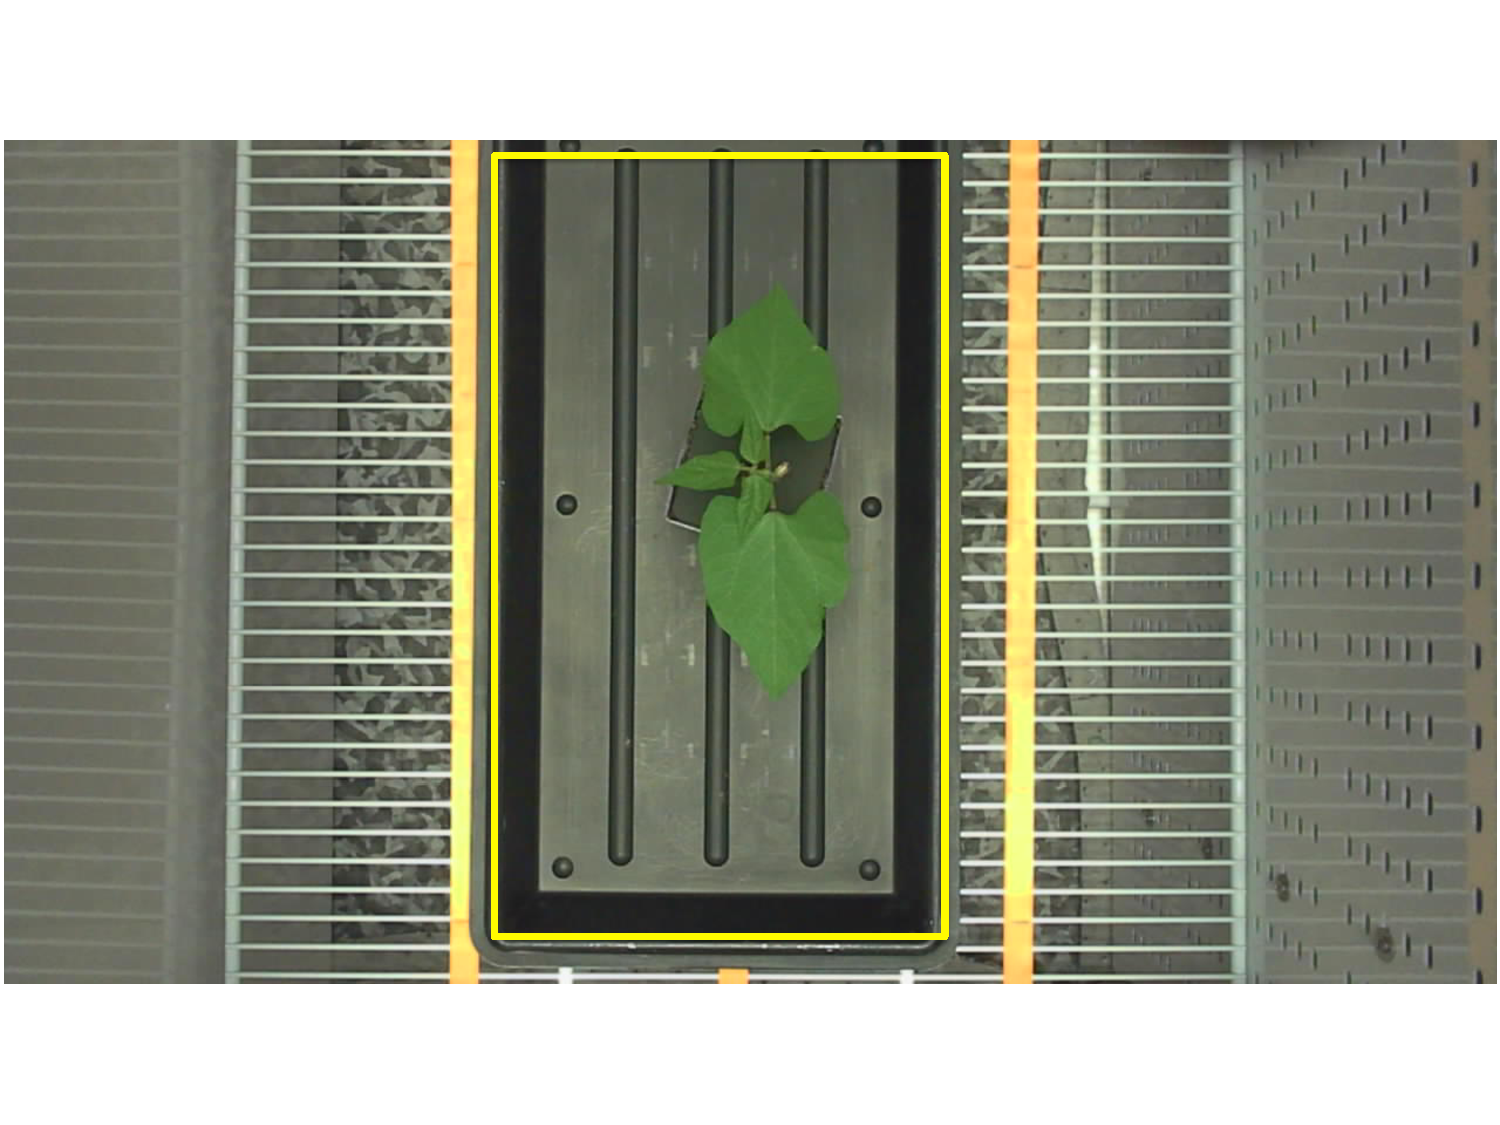
\includegraphics[width=.23\textwidth]{Figures/FourModalities/B_rgb}&
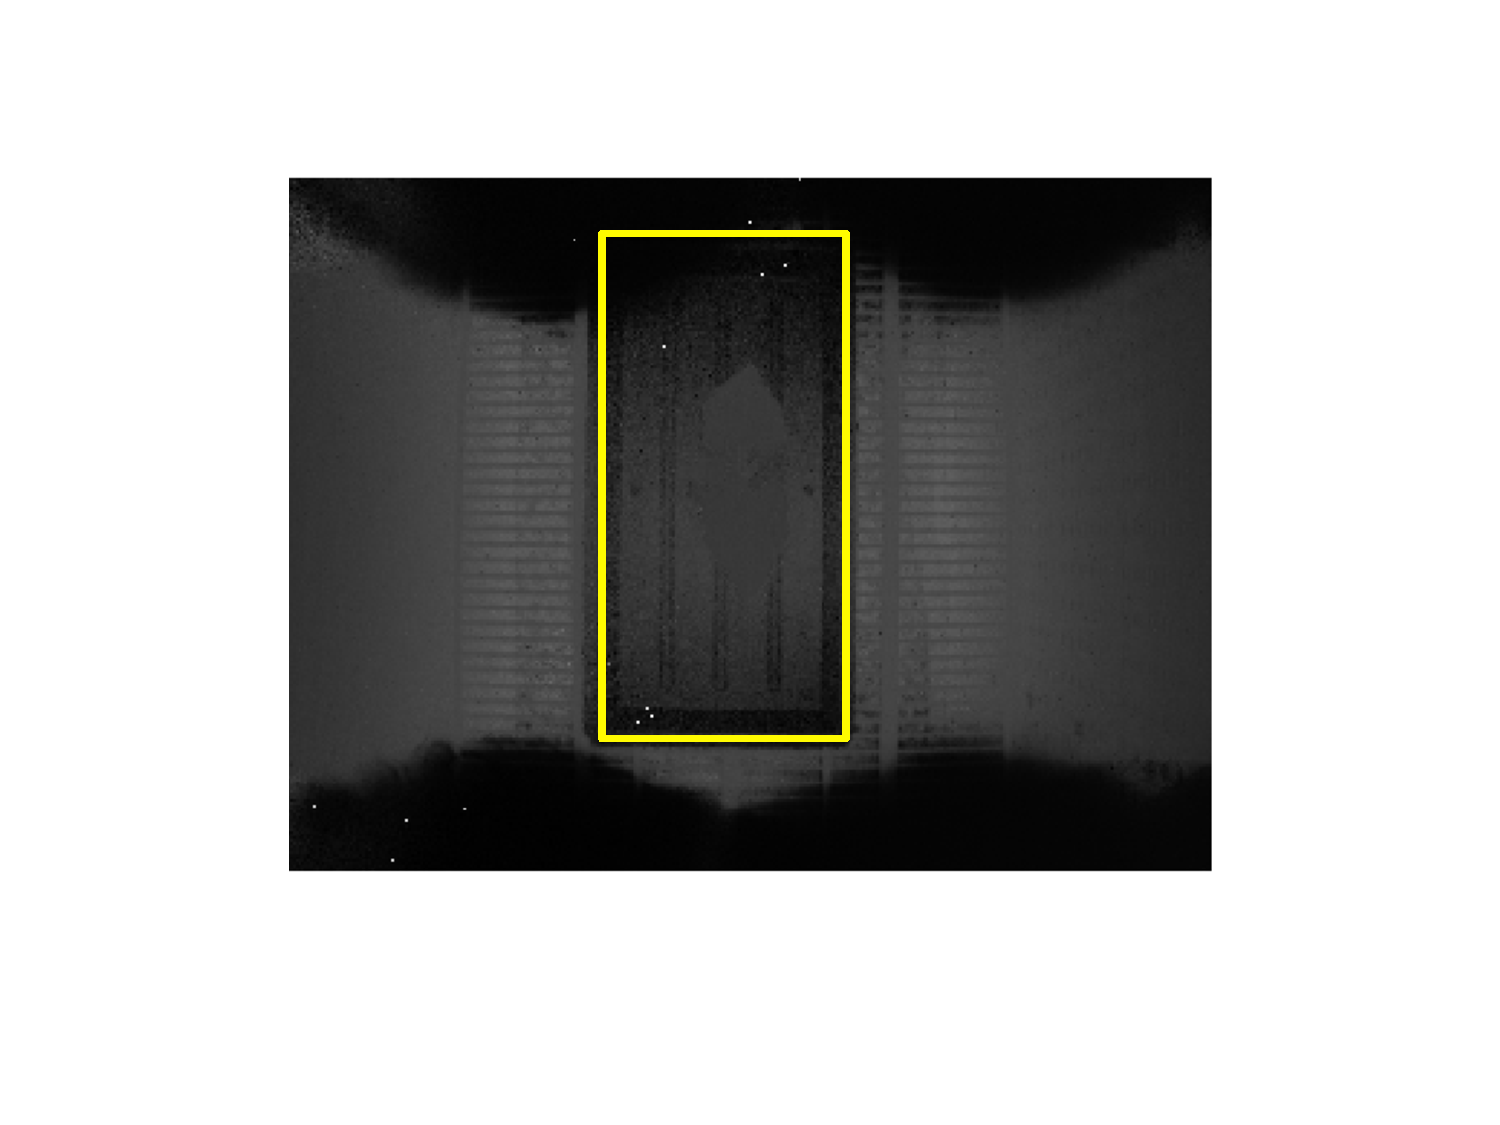
\includegraphics[width=.23\textwidth]{Figures/FourModalities/B_depth}&
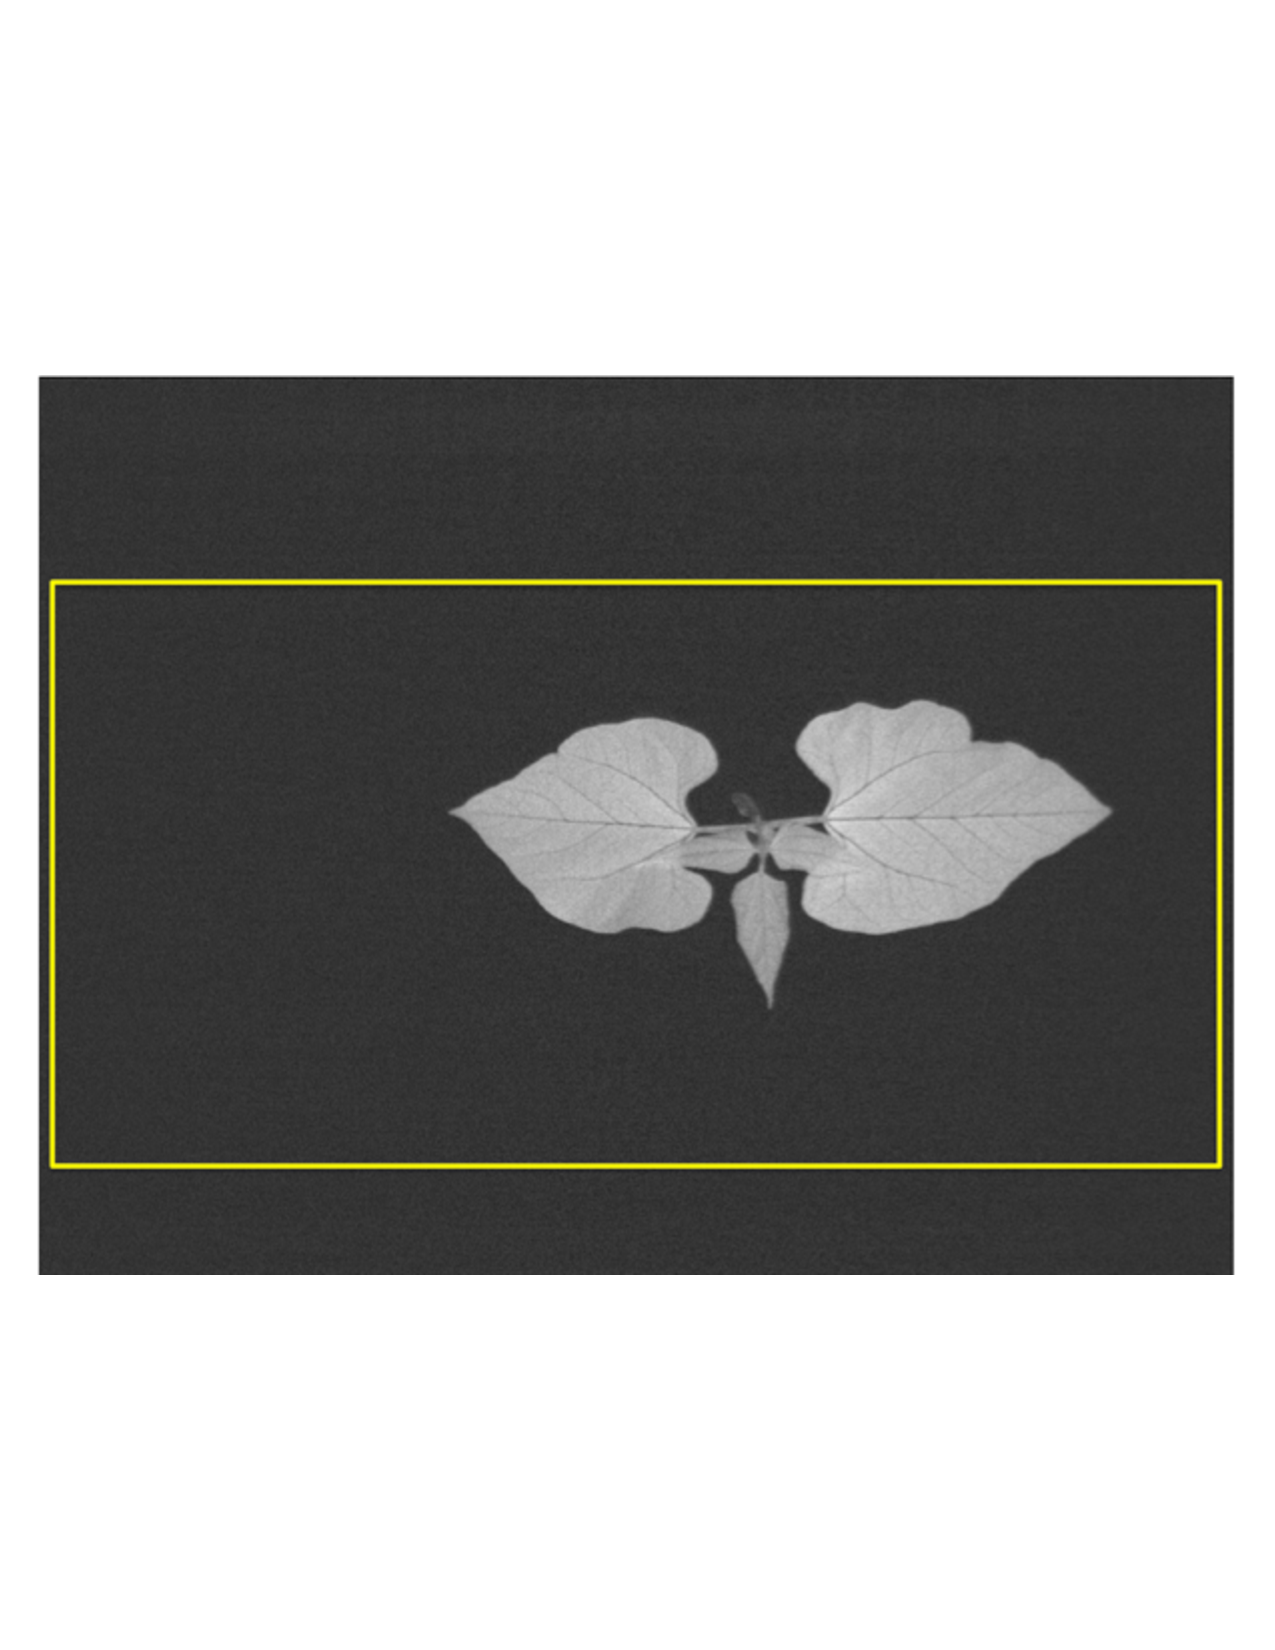
\includegraphics[width=.23\textwidth]{Figures/FourModalities/B_fmp}&
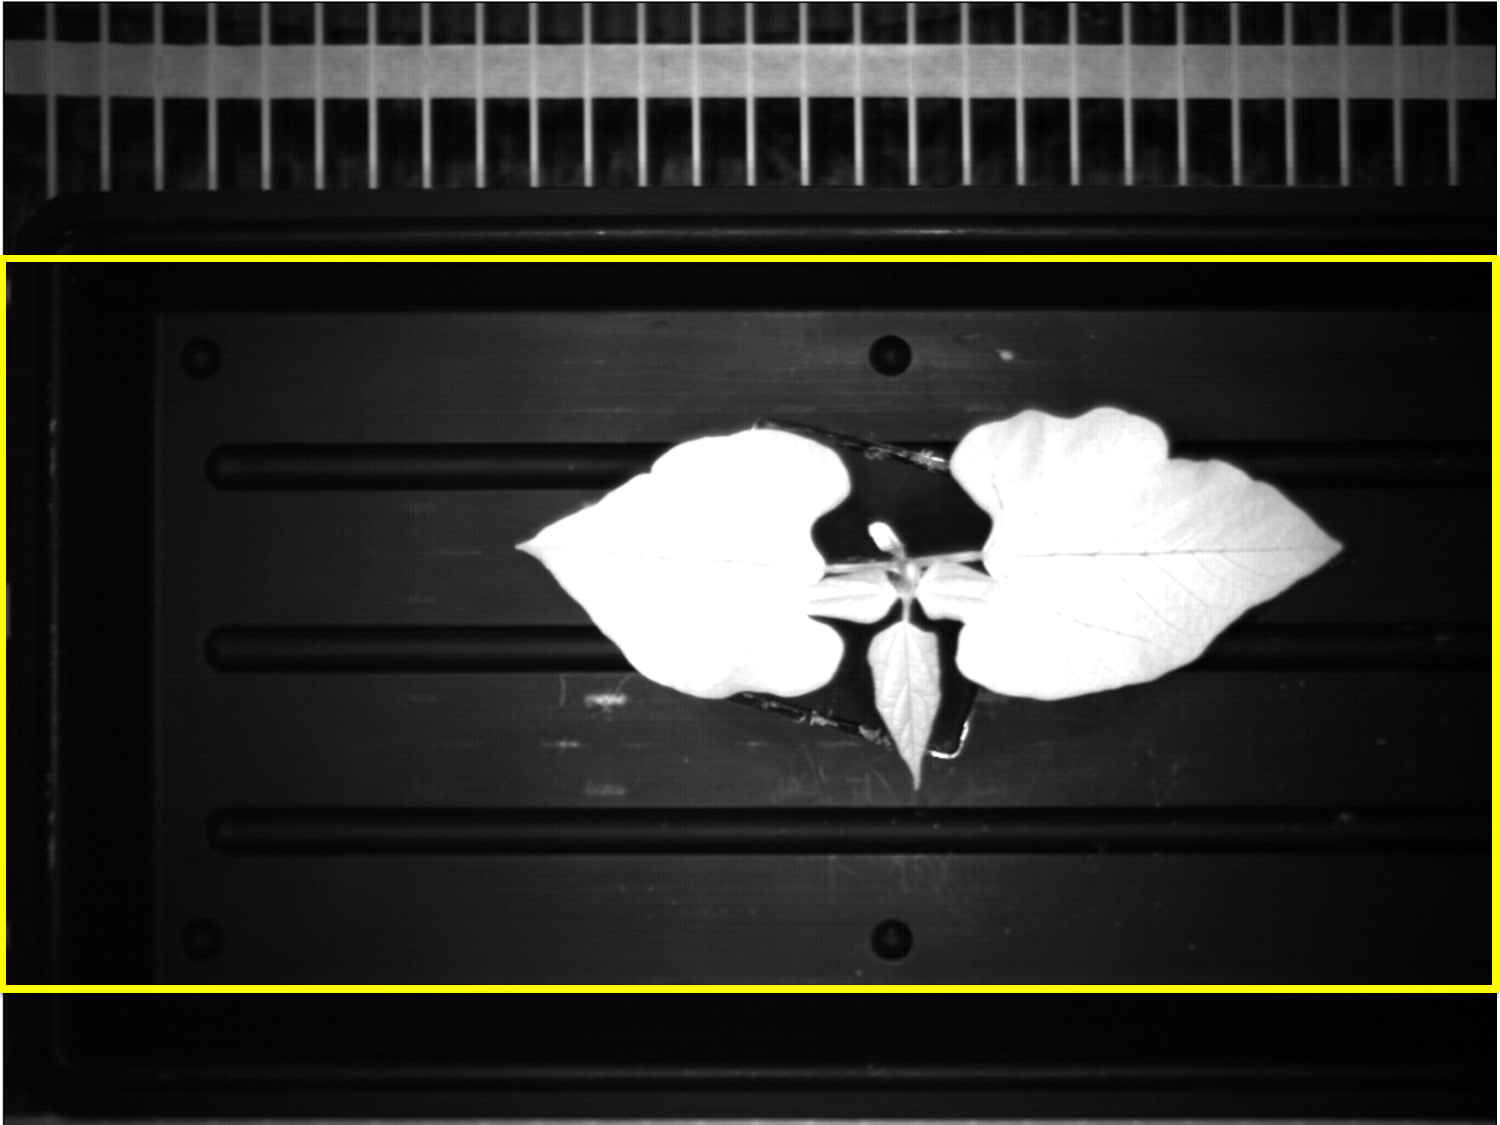
\includegraphics[width=.23\textwidth]{Figures/FourModalities/B_ir}\\
%(d) &
%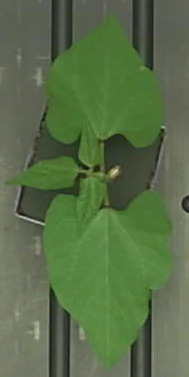
\includegraphics[width=.1\textwidth]{Figures/FourModalities/B1_rgb}&
%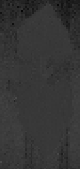
\includegraphics[width=.1\textwidth]{Figures/FourModalities/B1_depth}&
%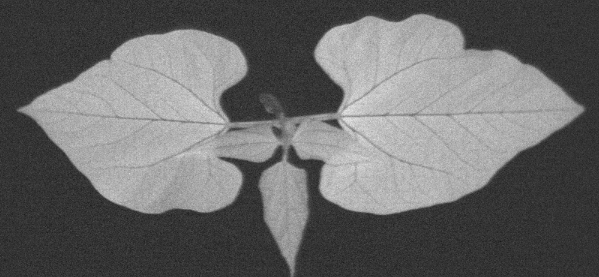
\includegraphics[width=.2\textwidth]{Figures/FourModalities/B1_fmp}&
%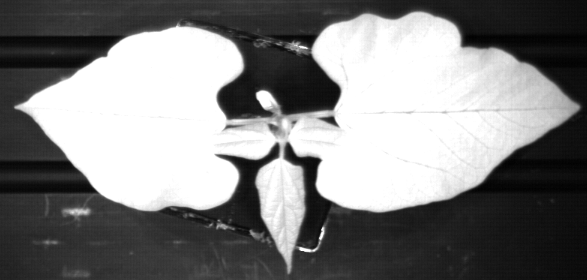
\includegraphics[width=.2\textwidth]{Figures/FourModalities/B1_ir}\\
%Bean: RGB & Bean: depth & Bean: fluorescence & Bean: IR \\
 & RGB & depth & fluorescence & IR\\
\end{tabular}
\caption{The multi-modality plant imagery database of MSU-PID. (a) four modalities of Arabidopsis; (b) zoom in view of Arabidopsis plant $1$; (c) four modalities of bean.}
\label{fig:fourmodality}
\end{centering}
\end{figure*}


Plants develop through a complex interaction between genotype and environment. 
This determines their structure, functions, and thus performance such as yield or efficient use of resources. 
In order to understand the genetic basis of these economically important parameters, it is essential to quantitatively assess plant phenotypes and then identify the latent relationships to genotypes and environmental factors.
%
Plant visual phenotyping has been performed by farmers and breeders for more than $5,000$ years. 
In the past, traditional phenotyping is based on experience and intuition, and is laborious~\cite{johannsenerblichkeit}. 
Recent progresses in imaging sensor, robotics and automation technologies lead to the development of the ever-increasing new field of highly automated, non-destructive {\it plant visual phenotyping}~\cite{furbank2011phenomics,cruz2015depi}. 
%Modern plant phenotyping is a comprehensive, large-scale assessment of plant traits such as growth, development, tolerance, resistance, architecture, physiology, ecology, yield, and metadata that form the basis for more complex parameters.
%
The objective of modern  plant visual phenotyping is to analyze and categorize the morphological characteristics of plants, and thus accurately quantifying plant traits. %It advances crop yield improvement and enables the systematic study of the environmental plasticity of plants. %
In this interdisciplinary field, scientists employ various imaging sensors to capture plants and design advanced algorithms to automatically analyze the captured plant imagery, with the purpose of raising testable biological hypotheses to solve problems related to growth, development, stress tolerance, resistance, and so on.
%
%In old days, plant phenotyping was conducted through manual visual observation~\cite{Erblichkeit1903}. Today, motivated by the increasing lower cost and increasing diversity of imaging sensors technologies, image-based automatic plant visual phenotyping is quickly growing into a desirable and viable solution~\cite{furbank2011phenomics,cruz2015depi}.
%
A key advance in visual phenotyping is the capability to non-invasively capture plant traits, enabling continuous measurements that are necessary to monitor plants during growth and/or under stress conditions. Vision based phenotyping also increases the throughput of phenotyping experiments by eliminating destructive operations. 
The increased capacity allows more genotypes or biological replicates to be examined under the same environmental conditions~\cite{fahlgren2015lights,walter2015plant}.

One practical goal of plant visual phenotyping is to accurately quantify plant traits, particularly those related to photosynthetic performance, growth, yield and resilience to environmental stress.  
For the approaches to be of practical use, plants must be monitored continuously, over developmental time scales and under conditions that more closely approximate the native environment (dynamic 'field' conditions)~\cite{fahlgren2015lights,walter2015plant}.
%
The capacity to identify and track individual leaves throughout experiments is important for more clearly defining phenotypic behaviors related to leaf specific factors such as developmental age~\cite{schottler2015photosynthetic} and/or following the application of stress. 
For example, decrease in the average photosynthetic efficiency ($\Phi_{II}$, quantum yield of photochemistry at photosystem II) of an Arabidopsis plant may reflect a heterogeneous distribution of $\Phi_{II}$ values across its entire photosynthetic surface area~\cite{oxborough2004imaging}. 
In this case, mapping distributions to individual leaves can be used to distinguish between a systemic (whole plant) effect and localization of the effect to subset leaves.
%
In addition, using more detailed information, such as leaf angle and height/position as well as canopy density/size, it should be possible to improve estimation of total photosynthetic capacity over time (particularly for plants with more complex canopies, like common bean or tobacco), since these factors influence absorption and availability of the light energy used to drive photosynthesis.

\begin{table*}[t!]
\centering
\begin{threeparttable}
\caption{Plant image databases.}
%\resizebox{12cm}{!} {
%\begin{tabular}{|l@{}|@{}c@{}|@{}c@{}|@{}c@{}|@{}c@{}|@{}c@{}|}
\begin{tabular}{l|c|c|c|c|c|c}
%\hline
%\multirow{2}{*}{Database}& \multirow{2}{*}{Modality} & \multirow{2}{*}{Applications}\tnote{a} & \multirow{2}{*}{Plant Type} & Subject/ &Total & Labeled \\
%& & & & Classe \# & Image \# & Image \# \\ \hline
%Swedish leaf~\cite{soderkvist2001computer} & Scaned leaf & LC& Swedish trees & $15$ & $1,125$ & $1,125$ \\ \hline
%Flavia~\cite{wu2007leaf} & RGB & LC& Leaves & $32$ & $2,120$ & $2,120$ \\ \hline
%Leafsnap~\cite{kumar2012leafsnap} & RGB & LC& USA trees & $184$ & $29,107$ & $29,107$ \\ \hline
%Crop/weed~\cite{haug2014crop} & RGB &Weed detection & Crop/weed & $2$ & $60$ & $60$ \\ \hline
%\multirow{2}{*}{LSC~\cite{haug2014crop}} & \multirow{2}{*}{RGB} & \multirow{2}{*}{LS, LO} & Arabidopsis & $43$ & $6287$ & $201$ \\ \cline{4-7}
%& & & Tobacco & $80$ & $165,120$ & $83$ \\ \hline
%\multirow{2}{*}{MSU-PID} & fluorescence, & LS, LO, & Arabidopsis & $16$ & $2304\times 4$ & $576\times 4$ \\ \cline{4-7}
%& IR, RGB, depth & LA, LT & Bean & $5$ & $350\times 4$ & $175\times 4$ \\ \hline
%\hline
\hline
\multirow{2}{*}{Database}& \multirow{2}{*}{Modality} & \multirow{2}{*}{Applications}\tnote{a} & \multirow{2}{*}{Plant Type} & Subject/ &Total & Labeled \\
& & & & Classe \# & Image \# & Image \# \\ \hline
Swedish leaf & \multirow{2}{*}{Scaned leaf} & \multirow{2}{*}{LC} & \multirow{2}{*}{Swedish trees} & \multirow{2}{*}{$15$} & \multirow{2}{*}{$1,125$} & \multirow{2}{*}{$1,125$} \\
~\cite{soderkvist2001computer} & & & & & & \\ \hline
Flavia & \multirow{2}{*}{RGB} & \multirow{2}{*}{LC} & \multirow{2}{*}{Leaves} & \multirow{2}{*}{$32$} & \multirow{2}{*}{$2,120$} & \multirow{2}{*}{$2,120$} \\
~\cite{wu2007leaf} & & & & & & \\ \hline
Leafsnap & \multirow{2}{*}{RGB} & \multirow{2}{*}{LC} & \multirow{2}{*}{USA trees} & \multirow{2}{*}{$184$} & \multirow{2}{*}{$29,107$} & \multirow{2}{*}{$29,107$} \\
~\cite{kumar2012leafsnap} & & & & & & \\ \hline
Crop/weed & \multirow{2}{*}{RGB} & \multirow{2}{*}{Weed detection} & \multirow{2}{*}{Crop/weed} & \multirow{2}{*}{$2$} & \multirow{2}{*}{$60$} & \multirow{2}{*}{$60$} \\
~\cite{haug2014crop} & & & & & & \\ \hline
LSC & \multirow{2}{*}{RGB} & \multirow{2}{*}{LS, LO} & Arabidopsis & $43$ & $6287$ & $201$ \\ \cline{4-7}
~\cite{haug2014crop} & & & Tobacco & $80$ & $165,120$ & $83$ \\ \hline
\multirow{2}{*}{MSU-PID} & fluorescence, & LS, LO, & Arabidopsis & $16$ & $2304\times 4$ & $576\times 4$ \\ \cline{4-7}
& IR, RGB, depth & LA, LT & Bean & $5$ & $350\times 4$ & $175\times 4$ \\ \hline
\hline
\end{tabular}
%}
\begin{tablenotes}
\footnotesize
\item[a] The abbreviation in ``Applications'' column is defined as Leaf Classification (LC), Leaf Segmentation (LS), Leaf Counting (LO), Leaf Alignment (LA), and Leaf Tracking (LT).
\end{tablenotes}
\end{threeparttable}
\label{tab:database}
\end{table*}

Due to diverse variations of leaf shape, appearance, layout, growth and movement, plant image analysis is a non-trivial computer vision task~\cite{Minervini2015}.
In order to develop advanced computer vision algorithms, image databases that are well representative of this application domain is highly important.
In fact, computer vision research lives on and advances with databases, as evidenced by the successful databases in the field (e.g., FERET~\cite{Phillips2000} and LFW~\cite{LFW}).
However, the publicly available database for plant phenotyping is still very limited, with the only exception of LSC database~\cite{scharr2014annotated}, which, nevertheless, has its own limitations on the type of images (RGB only) and is only suitable for a small set of plant image analysis applications.


To facilitate future research on plant image analysis, as well as remedy the limitation of existing databases in the field, this paper presents a newly collected multi-modality Plant Imagery Database through an interdisciplinary effort at Michigan State University (MSU), which is termed ``MSU-PID''.
As illustrated in Fig.~\ref{fig:fourmodality}, the MSU-PID database includes the imagery of two types of plants (Arabidopsis and bean, both are widely used in plant research) captured by four types of imaging sensors, i.e., fluorescence, infrared (IR), RGB color, and depth.
All four sensors are synchronized and are programmed to periodically capture imagery data for multiple consecutive days.
Checkerboard-based camera calibration is performed on each modality providing intrinsic camera parameters and poses.  In addition explicit correspondence between the pixels of {\it any} two modalities is obtained using an homographic warping of a plane through the plants.   


The type and amount of manual labels on a database is a critical enabler to the potential applications of the database.
For a subset of the MSU-PID database, we manually label the ground truth regarding the leaf identification number, locations of leaf tips, and leaf segments.
As a result, MSU-PID is suitable for a number of applications, including 1) {\it leaf segmentation} that aims at estimating the correct segmentation mask of each leaf in an image, 2) {\it leaf counting} that estimates the correct number of leaves within a plant, 3) {\it leaf alignment} that aligns the two tips of each leaf -- the cornerstone of the leaf structure, and 4) {\it leaf tracking} that is designed to track each leaf over time.
Finally, to provide a performance baseline for future research and comparison, we apply our automatic leaf segmentation framework~\cite{yin2014a,yin2014b} to the Arabidopsis imagery and demonstrate the unique challenge of image analysis on this database.

In summary, this paper and our database have made the following main contributions.
\begin{itemize}
\item MSU-PID is the first {\it multi-modality} plant image database. This allows researchers to study the strength and weakness of individual modality, as well as their various combinations in plant image analysis.
\item Our unique imaging setup and the variety of manual labels make MSU-PID an ideal candidate for evaluating a diverse set of plant image analysis applications including leaf segmentation, leaf counting, leaf alignment, leaf tracking, and potentially leaf growth prediction and $3$D leaf reconstruction.
\end{itemize}


